% mnras_template.tex
%
% LaTeX template for creating an MNRAS paper
%
% v3.0 released 14 May 2015
% (version numbers match those of mnras.cls)
%
% Copyright (C) Royal Astronomical Society 2015
% Authors:
% Keith T. Smith (Royal Astronomical Society)

% Change log
%
% v3.0 May 2015
%    Renamed to match the new package name
%    Version number matches mnras.cls
%    A few minor tweaks to wording
% v1.0 September 2013
%    Beta testing only - never publicly released
%    First version: a simple (ish) template for creating an MNRAS paper

%%%%%%%%%%%%%%%%%%%%%%%%%%%%%%%%%%%%%%%%%%%%%%%%%%
% Basic setup. Most papers should leave these options alone.
\documentclass[a4paper,fleqn,usenatbib]{mnras}

% MNRAS is set in Times font. If you don't have this installed (most LaTeX
% installations will be fine) or prefer the old Computer Modern fonts, comment
% out the following line
\usepackage{newtxtext,newtxmath}
% Depending on your LaTeX fonts installation, you might get better results with one of these:
%\usepackage{mathptmx}
%\usepackage{txfonts}

% Use vector fonts, so it zooms properly in on-screen viewing software
% Don't change these lines unless you know what you are doing
\usepackage[T1]{fontenc}
\usepackage{ae,aecompl}


%%%%% AUTHORS - PLACE YOUR OWN PACKAGES HERE %%%%%

% Only include extra packages if you really need them. Common packages are:
\usepackage{graphicx}	% Including figure files
\usepackage{amsmath}	% Advanced maths commands
\usepackage{amssymb}	% Extra maths symbols
\usepackage{deluxetable}


%%%%%%%%%%%%%%%%%%%%%%%%%%%%%%%%%%%%%%%%%%%%%%%%%%

%%%%% AUTHORS - PLACE YOUR OWN COMMANDS HERE %%%%%

% Please keep new commands to a minimum, and use \newcommand not \def to avoid
% overwriting existing commands. Example:
%\newcommand{\pcm}{\,cm$^{-2}$}	% per cm-squared

%%%%%%%%%%%%%%%%%%%%%%%%%%%%%%%%%%%%%%%%%%%%%%%%%%

%%%%%%%%%%%%%%%%%%% TITLE PAGE %%%%%%%%%%%%%%%%%%%

% Title of the paper, and the short title which is used in the headers.
% Keep the title short and informative.
\title[Mid-IR RR Lyrae PL Relation in $\omega$ Cen]{The Carnegie RR Lyrae Program: The Mid-Infrared RR Lyrae Period-Luminosity Relation in $\omega$ Centauri}

% The list of authors, and the short list which is used in the headers.
% If you need two or more lines of authors, add an extra line using \newauthor
\author[M. Durbin et al.]{
Meredith Durbin$^{1,2}$\thanks{E-mail: mdurbin@stsci.edu}
Victoria Scowcroft$^{3}$
Wendy Freedman$^{4}$
Gurtina Besla$^{5}$ 
\newauthor Giuseppe Bono$^{6, 7}$
Maria-Rosa Cioni$^{8, 9, 10}$
Gisella Glementini$^{11}$
Kathryn Johnston$^{12}$
\newauthor Nitya Kallivayalil$^{13}$
Juna Kollmeier$^{3}$
David Law$^{2}$
Barry Madore$^{3}$
Steve Majewski$^{13}$
\newauthor Roeland van der Marel$^{2}$
Massimo Marengo$^{14}$
Andrew~J.~Monson$^{3}$
David Nidever$^{15}$ 
Grzegorz Pietrzynski$^{16, 17}$
George Preston$^{3}$
Mark Seibert$^{3}$
Horace Smith$^{18}$
\newauthor Igor Soszynski$^{16}$
Ian Thompson$^{3}$
Andrzej Udalski$^{16}$
\\
% List of institutions
$^1$ Pomona College, Claremont, CA 91711, USA \\
$^2$ Space Telescope Science Institute, 3700 San Martin Drive, Baltimore, MD 21218, USA \\
$^3$ Observatories of the Carnegie Institution of Washington, 813 Santa Barbara St., Pasadena, CA 91101, USA \\
$^4$ Department of Astronomy and Astrophysics, University of Chicago, 5640 S Ellis Ave, Chicago, IL 60637, USA \\
$^5$ Department of Astronomy and Steward Observatory, University of Arizona, 933 North Cherry Avenue,   Tucson, AZ 85721, USA \\
$^6$ Univ. Roma ``Tor Vergata", Via della Ricerca Scientifica, 1 - 00133, Roma, Italy \\
$^7$ INAF-OAR, via Frascati 33 - 00040, Monte Porzio Catone (RM), Italy \\
$^8$ Universtat Potsdam, Institut fur Physik und Astronomie, Karl-Liebknecht-Str. 24/25, 14476 Potsdam, Germany \\
$^9$ Leibniz-Institut fur Astrophysik Potsdam, An der Sternwarte 16, 14482 Potsdam, Germany \\
$^{10}$ University of Hertfordshire, Physics, Astronomy and Mathematics, College Lane, Hatfield AL10 9AB, United Kingdom \\
$^{11}$ INAF - Osservatorio Astronomico, Via Ranzani n. 1, 40127 Bologna, Italy \\
$^{12}$ Department of Astronomy, Columbia University, New York, NY 10027, USA  \\
$^{13}$ Department of Astronomy, University of Virginia, Charlottesville, VA 22904-0818, USA \\
$^{14}$ Department of Physics and Astronomy, Iowa State University, Ames, IA, USA \\
$^{15}$ Department of Astronomy, University of Michigan, Ann Arbor, MI 48109, USA \\
$^{16}$ Warsaw University Observatory Al. Ujazdowskie 4, 00-478 Warszawa, Poland \\
$^{17}$ Departamento de Astronomia, Universidad de Concepcion, Casilla 160-C, Chile \\
$^{18}$ Department of Physics and Astronomy, Michigan State University, East Lansing, MI, USA 48824 \\
}

% These dates will be filled out by the publisher
\date{Accepted XXX. Received YYY; in original form ZZZ}

% Enter the current year, for the copyright statements etc.
\pubyear{2015}

% Don't change these lines
\begin{document}
\label{firstpage}
\pagerange{\pageref{firstpage}-\pageref{lastpage}}
\maketitle

% Abstract of the paper
\begin{abstract}
Something something metallicity
%We present new period-luminosity relations for RR Lyrae variables in 3.6 and 4.5 \micron\ derived from time-resolved IRAC data of $\omega$ Centauri. The sample consists of 36 RR Lyrae in 3.6 \micron\ and 37 in 4.5 \micron, 22 of which appear in both channels and have literature values for metallicities. We find no compelling evidence for a metallicity correlation in the residuals, based on a spread of 1.2 dex in [Fe/H].
\end{abstract}

% Select between one and six entries from the list of approved keywords.
% Don't make up new ones.
\begin{keywords}
keyword1 - keyword2 - keyword3
\end{keywords}

%%%%%%%%%%%%%%%%%%%%%%%%%%%%%%%%%%%%%%%%%%%%%%%%%%

%%%%%%%%%%%%%%%%% BODY OF PAPER %%%%%%%%%%%%%%%%%%

\section{Introduction}
\label{sec:intro}
The Carnegie Hubble Program (CHP) is a Warm \textit{Spitzer} program with the aim of measuring $H_{0}$ to a systematic uncertainty of 3\%, eventually reducing that uncertainty to 2\% using \textit{JWST}. The first part of the CHP used Cepheids as the primary distance indicator, using parallax measurements of Cepheids from \textit{HST} \citep{2007AJ....133.1810B} to calibrate the zero-point of the Cepheid Period-Luminosity (PL) relation (also known as the Leavitt Law, or LL), leading out to Cepheid measurements in the Milky Way \citep[MW,][]{2012ApJ...759..146M} and Large Magellanic Cloud \citep[LMC,][]{2011ApJ...743...76S}. An initial recalibration of $H_{0}$ from CHP was presented in \citet{2012ApJ...758...24F}.

The CHP removed many systematics from the $H_{0}$ measurement by moving to the mid-infrared (extinction is reduced by a factor of 16 to 20, amplitude of Cepheid pulsation is reduced, intrinsic width of LL is reduced) and by using a single instrument (no effects from ground-to-space transformation, for example) but there are some effects that cannot be accounted for without further tests. By only using a single distance indicator (i.e. Cepheids) for the zero-point measurement, we have no understanding of the intrinsic accuracy of our measurement. With recent measurements from cosmic microwave background (CMB) experiements such as Planck \citep{2015arXiv150201589P} in tension with local $H_{0}$ values, we must assess all possible sources of systematic uncertainty in our measurement. This is where the Carnegie RR Lyrae Program comes into play.

** VS NOTE: With regard to CMB - is measurements the correct word here? Obviously Planck et al. make measurements, but they do not measure $H_{0}$, it is inferred from a model. What word would be more appropriate here? **

The Carnegie RR Lyrae Program (CRRP) assess a systematic that was unreachable in the original CHP -- the intrinsic accuracy of the mid-infrared Cepheid standard candle distance scale when compared to the standard ruler distance scale of CMB and Baryon Acoustic Oscillation (BAO) measurements. With only one ``test candle'' it is impossible to make any assessment of this accuracy. However, when we have two standard candles with similar precision we can make meaningful comparisons and assess the systematic accuarcy of both of them.

In the past RR Lyrae variables have often been thought of as the poor substitute for Cepheids in terms of distance scale measurements. They are intrinsically fainter, and in the optical follow a much shallower, even horizontal, PL relation. Determining an accurate distance to an RR Lyrae (RRL) in the $V$ band requires knowledge of its [Fe/H] -- a quantity which itself is not  easy to obtain. However, in more recent years near- and mid-infrared observations have shown the true power of RRL as precision distance indicators. In a similar vein to Cepheids, \text{HST} parallaxes were obtained for serveral Galactic RRL calibrators \citet{2011AJ....142..187B} and several groups have been studying the populations of RRL in globular clusters and nearby dwarf spheroidal galaxies (NEED REFS). 

In the mid-infrared RRL exhibit similar properties to Cepheids\citep{2013ApJ...776..135M}. Their light curve amplitudes are minimised as we are seeing deeper into the star. At the wavelengths observed by Warm \textit{Spitzer} (3.6 and 4.5~$\mu$m) we do not see photospheric effects, but only the effects of temperature driving the pulsation. Essentially, the mid-infrared light curve is tracing the radius change of the star. A by-product of this effect is that the intrinsic width of the RRL PL relation is also minimised in the mid-infrared (mid-IR). The PL relation for pulsational variables can be thought of as a two-dimensional projection of the three-dimensional period-luminosity-colour relation (see figure 3 of \citet{1991PASP..103..933M} for a graphical representation). As the colour-width decreases in the mid-IR, the width of the PL naturally decreases. As one moves from the optical to the mid-IR, the slope of the PL relation steepens and its dispersion dramatically decreases; this phenomenon has been demonstrated in simulations by \citet{2004ApJS..154..633C}, and by several observational efforts, as illustrated in fig. 4 of \citet{2013ApJ...776..135M}. The slope should asymptotically approach the predicted slope of the period-radius relation, resulting in a slope between $-2.4$ and $-2.8$. Through this decrease in dispersion we have found that the intrinsic width of the mid-IR PL for RRL is in fact smaller than for Cepheids -- 0.05~mag compared to 0.10~mag (Monson et al. 2015, Neely et al. 2015). This translates to an uncertainty on an individual RR Lyrae star of 2\%, compared to 4\% for Cepheids. 

In this work we present the mid-IR PL relation for the RRL in the $\omega$~Cen Galactic Globular Cluster (GGC). 
Here we present a mid-infrared of the RR Lyrae period-luminosity (PL) relation in the IRAC channels 1 and 2 centered on 3.6 and 4.5 \micron\ respectively, as well as a preliminary investigation into metallicity effects on the PL relation.

There are very few metallic or molecular transition lines in the mid-IR at typical RR Lyrae temperatures, so the effects of metallicity on luminosity should be minimized. However, $\omega$~Cen provides the ideal test bed for any effect that we may not have predicted. Such an effect is not out of the realm of possibility; for example, the CO band head at 4.5~$\mu$m has been found to have a significant dependence on metallicity, and has such prevented the IRAC 4.5~$\mu$m Cepheid observations from being used for distance measurements in the CHP. As our concern in this program is systematic precision, we must ensure that similar effects do not plague the RRL distance scale.  

$\omega$ Cen in particular is ideal for calibrating the RR Lyrae period-luminosity-metallicity relation, as it contains 192 known RR Lyrae \citep{2004A&A...424.1101K} with a metallicity range spanning over 1.5 dex (Bono 2013, private communication); a metallicity spread this wide is not found in any other GGC. As noted in \citet{2006MNRAS.372.1675S}, one of the advantages of using globular clusters to calibrate PL coefficients is that all stars in a cluster can be considered to be at the same distance from Earth. We can therefore assume that any dispersion in the PL relation is a combination of the a) the intrinsic dispersion of the PL relation, b) the photometric uncertainties, and c) dispersion induced by the spread in metallicity of the RRL. We have measured the intrinsic dispersion of the RRL PL from other clusters (e.g. M4, Neely et al. 2015), and our photometric uncertainties are a well defined \textbf{constraint, value?? what is the correct word?}, so the only unknown in this problem is the dispersion due to the spread in metallicity of the cluster. We are lucky with $\omega$~Cen that we can also take a second approach to establishing the metallicity effect on the RRL PL relation. As it is such a unique object, $\omega$~Cen is extremely well studied and many of its RRL have spectroscopic or photometric metallicities available. As another test of the effect of metallicity, we use these measeurements to assess the $\gamma$ parameter for the GGC, where 
\begin{equation} \label{eqn:gamma}
\gamma = \dfrac {\Delta \text{mag}} {[Fe/H]}\text{,}
\end{equation}

similar to $\gamma$ used to quantify the effect of metallicity on the zero-point of the Cepheid PL relation. 

The paper is set out as follows: Section~\ref{sec:observations} details the observations and data reduction. Section~\ref{sec:pl_relation} describes the mid-IR PL relations and Section~\ref{sec:distance_moduli} discusses the application of these to a distance measurement of  $\omega$~Cen. Section~\ref{sec:metallicity} and Section~\ref{sec:discussion} examine the effect of metallicity on mid-IR observations of RR Lyrae variables and its implications for distance measurements and the extragalactic distance scale. In Section~\ref{sec:conclusions} we present our conclusions.


\section{Observations \& Data Reduction}
\label{sec:observations}
The observations for this work were taken as part of the Warm~\textit{Spitzer} mission as part of the Carnegie RR Lyrae Program (PI W. Freedman, PID 90002). Three fields in $\omega$~Cen were chosen; their positions and the positions of known RR Lyrae are shown in Figure~\ref{fig:omegaCen_fields}. To obtain optimal RRL light curves we chose to observe each field twelve times over approximately 16 hours, roughly corresponding to the period of the longest period RRL we expected to observe in the field. The observations of all three fields were taken on 2013-05-10 and 2013-05-11. Each field was observed using IRAC \citep{2004ApJS..154...10F} with a 30s frame time with a medium scale, gaussian 5-point dither pattern to mitigate any image artifacts. Images were collected in both the 3.6 and 4.5~$\mu$m channels. 

The science images were created using \textsc{mopex} \citep{2006SPIE.6274E..0CM}, first running overlap correction on the corrected BCDs (cBCDs) then mosaicking them at 0.6 arcsec pixel scale using the drizzle algorithm. Mosaicked location-correction images were created at the same time. 

[This paragraph is shamelessly lifted from the SMC paper I will fix this]
The data were reduced in an almost identical manner to the LMC data in Scowcroft (2011) [citation], with one significant difference; the full details of the photometry process can be found in that paper. The only difference in the data reduction process used here is that an empirically derived Point Response Function (PRF) was used rather than a model PRF, as the data were mosaicked to a nonstandard pixel scale. The PRF was derived from a set of [manually selected?] stars in field 2 (shown in Figure~\ref{fig:omegaCen_fields}), the least crowded field of the observations. As all observations were taken within 24 hours of each other, we expect little to no variation in the PRF between fields, and so find it acceptable to use the field 2 PRF for all photometry. Our photometry is calibrated to the standard system set by Reach et al. (2005).

\begin{figure}
\begin{center}
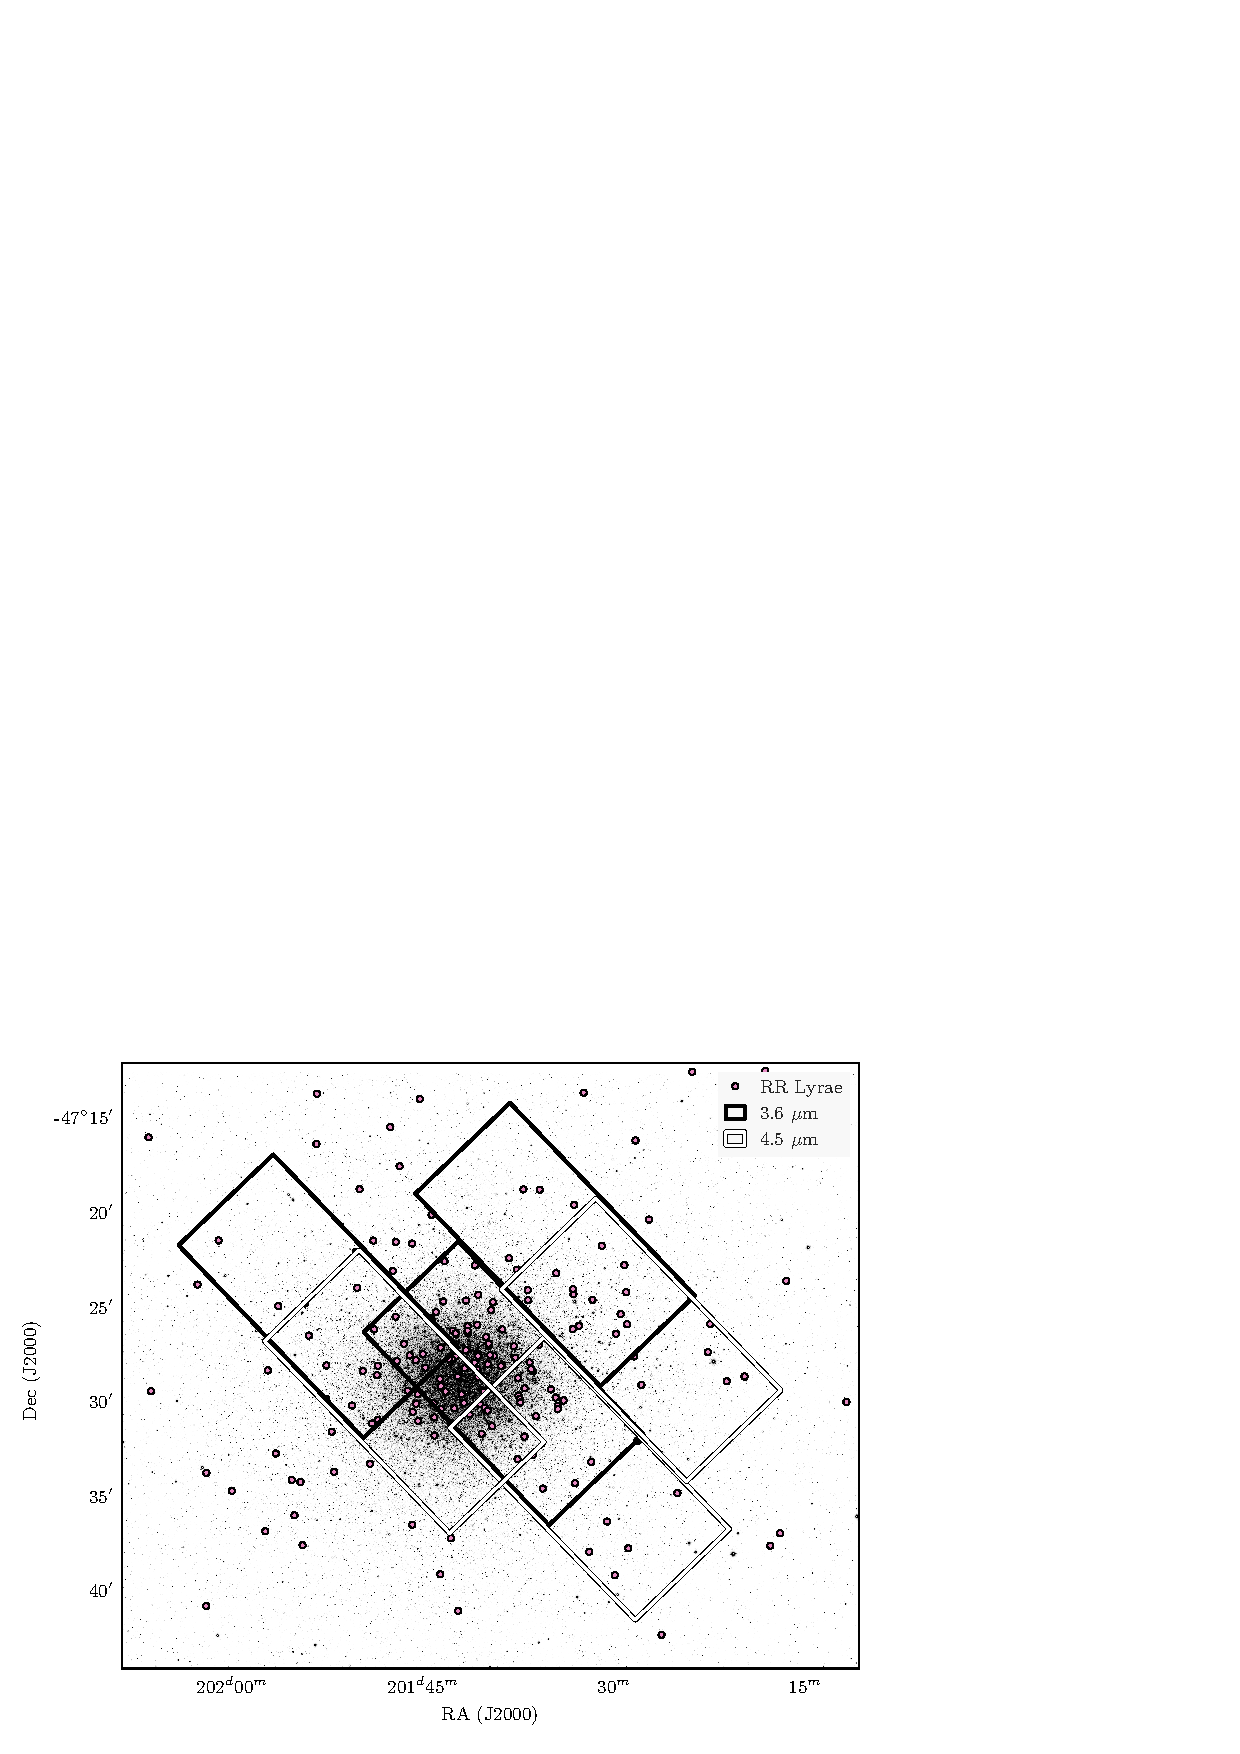
\includegraphics[width=80mm]{final_plots/omegacen_coverage_map.pdf}
\caption{A $K$-band image of $\omega$ Centauri from the FourStar camera, overlaid with the catalog of RR Lyrae (Kaluzny et. al. 2004) and footprints of the three IRAC fields.}
\label{fig:omegaCen_fields}
\end{center}
\end{figure}


%PSF photometry was performed in PyRAF 2.0 using the \textsc{daophot} package. Initial aperture photometry was performed with an aperture radius of 3.6\arcsec and annulus radius of 4.8\arcsec, whereas the standard IRAC aperture is 6\arcsec; a correction factor of 1.12841 and 1.12738 for 3.6 and 4.5 \micron\ respectively was applied to the instrumental magnitudes. We also calibrate the magnitudes from images in counts (required for \textsc{daophot}) back to flux magnitudes by performing aperture photometry on a set of bright, isolated stars in the flux images, finding the mean difference between the aperture flux magnitudes and PSF counts magnitudes of the same stars, and subtracting said difference from all PSF magnitudes. We also correct for location in the frame using the mosaicked correction images created by \textsc{mopex}

The primary limiting factor in this data is crowding: 77 RR Lyrae out of the original catalog of 192 (Kaluzny et al. 2004) [citation] were rejected due to crowding. To decide which stars to reject, a $K$-band image from the FourStar infrared camera on the \textit{Magellan} telescope at Las Campanas Observatory was used, as it provided a full view of the entire cluster at several times the resolution of \textit{Spitzer}, and the most crowded regions were more obvious than in the \textit{Spitzer} data, although the bandpasses are close enough that they are still comparable. The selection of which stars to reject was made on a primarily visual basis. % is there a way to make this whole thing sound less silly?

[Can someone who knows more about the fourstar photometry talk about that?]

\section{Period-Luminosity Relations}
\label{sec:pl_relation}

Our final photometry catalog is comprised of 24 RR Lyrae (11 fundamental mode and 13 first overtone) that appear in all five bandpasses. We use the near- and mid-infrared PL relation parameters presented in Tizio et al. (2015, in prep) [is this the right thing to cite? it's the last thing I can find in my email] as fiducial in all of our PL fitting. The relations take the form
\begin{equation}M = a + b\times\log P + c\times[Fe/H]\end{equation}
where $a$, $b$, and $c$ are theoretically derived coefficients.
With the use of these coefficients, the distance modulus becomes the only free parameter in our fit. We fit all distance moduli using a weighted least-squares method.

[table of PL parameters here]

For the metallicity term, not all stars in our sample have known metallicity values; thus we use an average metallicity value for all RR Lyrae in the cluster. We use both photometric (Rey et al 2000) [citation] and spectroscopic (Sollima et al 2006) [citation] metallicities for comparison. We find that there is little correspondence between individual metallicity measurements for stars which have both spectroscopic and photometric metallicity values, as shown in Figure~\ref{fig:metallicity_comparison}, and that the average metallicities of the spectroscopic and photometric catalogs differ by nearly 0.1 dex. We use a mean photometric [Fe/H] of  $-1.584$ and a spectroscopic [Fe/H] of $-1.677$.



\section{Distance Moduli}
\label{sec:distance_moduli}

[Again, shamelessly lifted from the SMC paper]
The five bands for which distance moduli are available can be combined to produce an estimate of the mean $E(B - V)$ and mean reddening-corrected distance modulus of the galaxy. We assume the ratio of total to selective absorption, $R_V = 3.1$, and fit three reddening laws simultaneously. For the near-infrared bands we use the appropriate relation from Cardelli et al. (1989) and for the mid-infrared we use the relation from Indebetouw et al. (2005). The relations are fit by minimizing the dispersion of the distance moduli around the values predicted by the reddening law. The resulting fits are shown in Figures~\ref{fig:omegaCen_dist_phot} and \ref{fig:omegaCen_dist_spect}.

The difference between the distance moduli derived from using spectroscopic and photometric metallicities respectively is less than 0.02 mag, well within the $\pm 0.053$ mag errors for each distance modulus; thus we can say that despite the disagreement between individual metallicity values, for our purposes there is no significant difference between the photometric and spectroscopic metallicity catalogs.

We find a true mean distance modulus of $\mu_0 = 13.686 \pm 0.053$ [is it cool to just average them], which is in excellent agreement with prior measurements using near-infrared RR Lyrae period-luminosity relations (Del Principe et al. 2006) and and the eclipsing binary OGLEGC17 (Thompson et al 2000), but significantly higher than the distances measured by dynamical modeling (Watkins et al 2013, van de Ven et al 2006). 

\section{Metallicity}
\label{sec:metallicity}

If there is any correlation between [Fe/H] and the PL residuals, we expect it to be a linear one, consistent with the theoretical metallicity terms $c\times[Fe/H]$. We fit a relation of the form
\begin{equation}\Delta[\lambda] = c\times[Fe/H] + d\end{equation}
to the 3.6~$\mu$m and 4.5~$\mu$m PL residuals and metallicity values for stars with individual metallicity values, as shown in Figures~\ref{fig:delta_3p6_phot}, \ref{fig:delta_3p6_spect}, \ref{fig:delta_4p5_phot}, and \ref{fig:delta_4p5_spect}. Relations were fit without weighting individual errors in either $\Delta[\lambda]$ or [Fe/H]. Although there are relatively large errors in both variables, they are consistent enough that weighting by errors would result in a fit heavily skewed by the few data points with low errors.

\section{Discussion}
\label{sec:discussion}

We find that although the scatter in the 3.6~$\mu$m and 4.5~$\mu$m PL relations is higher for $\omega$ Centauri than it is for M4 [citation], there is no evidence that it is due to metallicity. When we fit a line to [Fe/H] vs. $\Delta$3.6~$\mu$m and $\Delta$4.5~$\mu$m, both slopes are within $2\sigma$ of zero, indicating that there is no significant metallicity dependence in the PL residuals. When the outlier in [Fe/H] vs. 3.6~$\mu$m at [Fe/H] = $-2.0$ is removed from the photometric metallicities, the slopes of [Fe/H] vs. 3.6~$\mu$m and 4.5~$\mu$m both move within $1\sigma$ of zero.

Alternative explanations for the increased scatter relative to M4 include crowding and [other things here].


\section{Conclusions}
\label{sec:conclusions}


\section*{Acknowledgements}
\label{sec:acknowledgements}
This work is based on observations made with the Spitzer Space Telescope, which is operated by the Jet Propulsion Laboratory, California Institute of Technology under a contract with NASA. Support for this work was provided by NASA through an award issued by JPL/Caltech.


%%%%%%%%%%%%%%%%%%%%%%%%%%%%%%%%%%%%%%%%%%%%%%%%%%

%%%%%%%%%%%%%%%%%%%% REFERENCES %%%%%%%%%%%%%%%%%%

% The best way to enter references is to use BibTeX:

\bibliographystyle{mnras}
\bibliography{omegaCen_2015}
 % if your bibtex file is called example.bib


% Alternatively you could enter them by hand, like this:
% This method is tedious and prone to error if you have lots of references

%%%%%%%%%%%%%%%%%%%%%%%%%%%%%%%%%%%%%%%%%%%%%%%%%%

%%%%%%%%%%%%%%%%% APPENDICES %%%%%%%%%%%%%%%%%%%%%

\begin{figure}
\begin{center}
\includegraphics[width=80mm]{final_plots/multiwavelength_PL_samestars_spect.pdf}
\caption{PL relations for $J\!H\!K$, 3.6~$\mu$m, and 4.5~$\mu$m photometry using the average spectroscopic metallicity from Sollima et al. (2006) [cite].}
\label{fig:omegaCen_pl_spect}
\end{center}
\end{figure}

\begin{figure}
\begin{center}
\includegraphics[width=80mm]{final_plots/multiwavelength_PL_samestars_phot.pdf}
\caption{PL relations for $J\!H\!K$, 3.6~$\mu$m, and 4.5~$\mu$m photometry using the average photometric metallicity from Rey et al. (2000) [cite].}
\label{fig:omegaCen_pl_phot}
\end{center}
\end{figure}


\begin{figure}
\begin{center}
\includegraphics[width=80mm]{final_plots/metallicity_comparison_all.pdf}
\includegraphics[width=80mm]{final_plots/metallicity_comparison_samestars.pdf}
\caption{Spectroscopic vs. photometric measurements of [Fe/H] for the same RR Lyrae stars in $\omega$ Centauri. Top: every star for which both catalogs have [Fe/H] measurements. Bottom: only the stars which appear in our sample and have [Fe/H] measurements in both catalogs.}
\label{fig:metallicity_comparison}
\end{center}
\end{figure}

\begin{figure}
\begin{center}
\includegraphics[width=80mm]{final_plots/multiwavelength_distance_samestars_phot.pdf}
\caption{Distance moduli for $J\!H\!K$, 3.6~$\mu$m, and 4.5~$\mu$m photometry using the average photometric metallicity from Rey et al. (2000) [cite].}
\label{fig:omegaCen_dist_phot}
\end{center}
\end{figure}

\begin{figure}
\begin{center}
\includegraphics[width=80mm]{final_plots/multiwavelength_distance_samestars_spect.pdf}
\caption{Distance moduli for $J\!H\!K$, 3.6~$\mu$m, and 4.5~$\mu$m photometry using the average spectroscopic metallicity from Sollima et al. (2006) [cite].}
\label{fig:omegaCen_dist_spect}
\end{center}
\end{figure}

\begin{figure}
\begin{center}
\includegraphics[width=80mm]{final_plots/deltadelta_3p6_4p5_spect.pdf}
\caption{$\Delta$~3.6~$\mu$m vs. $\Delta$~4.5~$\mu$m using spectroscopic metallicities}
\label{fig:deltadelta_spect}
\end{center}
\end{figure}


\begin{figure}
\begin{center}
\includegraphics[width=80mm]{final_plots/delta_feh_3p6_phot.pdf}
\caption{[Fe/H] vs. $\Delta$~3.6~$\mu$m using photometric metallicities}
\label{fig:delta_3p6_phot}
\end{center}
\end{figure}

\begin{figure}
\begin{center}
\includegraphics[width=80mm]{final_plots/deltadelta_3p6_4p5_phot.pdf}
\caption{$\Delta$~3.6~$\mu$m vs. $\Delta$~4.5~$\mu$m using photometric metallicities}
\label{fig:deltadelta_phot}
\end{center}
\end{figure}

\begin{figure}
\begin{center}
\includegraphics[width=80mm]{final_plots/delta_feh_3p6_spect.pdf}
\caption{[Fe/H] vs. $\Delta$~3.6~$\mu$m using spectroscopic metallicities}
\label{fig:delta_3p6_spect}
\end{center}
\end{figure}

\begin{figure}
\begin{center}
\includegraphics[width=80mm]{final_plots/delta_feh_4p5_phot.pdf}
\caption{[Fe/H] vs. $\Delta$4.5~$\mu$m using photometric metallicities}
\label{fig:delta_4p5_phot}
\end{center}
\end{figure}

\begin{figure}
\begin{center}
\includegraphics[width=80mm]{final_plots/delta_feh_4p5_spect.pdf}
\caption{[Fe/H] vs. $\Delta$4.5~$\mu$m using spectroscopic metallicities}
\label{fig:delta_4p5_spect}
\end{center}
\end{figure}


%%%%%%%%%%%%%%%%%%%%%%%%%%%%%%%%%%%%%%%%%%%%%%%%%%


% Don't change these lines
\bsp	% typesetting comment
\label{lastpage}
\end{document}

% End of mnras_template.tex